% turbo-sc10-parametric.tex

\section{Subsonic compressor blade -- PyFun version}
%
This is the same flow specification as for the previous example but we directly 
use the functional form of the Standard Configuration 10 from \url{http://rpmturbo.com/testcases/sc10/index.html}.

In the input script, the blade surfaces are defined using \texttt{PyFunctionPath} 
objects that receive the functions \texttt{sc10\_top\_rotated} and 
\texttt{sc10\_bottom\_rotated}. These functions are created by rotating the original 
\texttt{sc10\_top} and \texttt{sc10\_bottom} functions by the blade stagger angle, 
using the \texttt{cfpylib.geom.transform\_pyfunc} library. Shell scripts and 
user defined boundary condition files are the same as for the previous example.

\begin{figure}[htbp]
\begin{center}
\includegraphics[width=0.9\textwidth,viewport=24 495 570 817]{../2D/turbo_sc10_parametric/mesh.pdf}
\end{center}
\caption{Mesh around the subsonic compressor blade.}
\label{turbo-sc10-parametric-meshfig}
\end{figure}

\begin{figure}[htbp]
\begin{center}
\includegraphics[width=0.9\textwidth,viewport=24 495 570 817]{../2D/turbo_sc10_parametric/mach-field.pdf}
\end{center}
\caption{Mach number field for flow over a subsonic compressor blade.}
\label{turbo-sc10-parametric-mach-fig}
\end{figure}

\begin{figure}[htbp]
\begin{center}
\includegraphics[width=0.9\textwidth,viewport=24 495 570 817]{../2D/turbo_sc10_parametric/pressure-field.pdf}
\end{center}
\caption{Pressure field for flow over a subsonic compressor blade.}
\label{turbo-sc10-parametric-pressure-fig}
\end{figure}

\begin{figure}[htbp]
\begin{center}
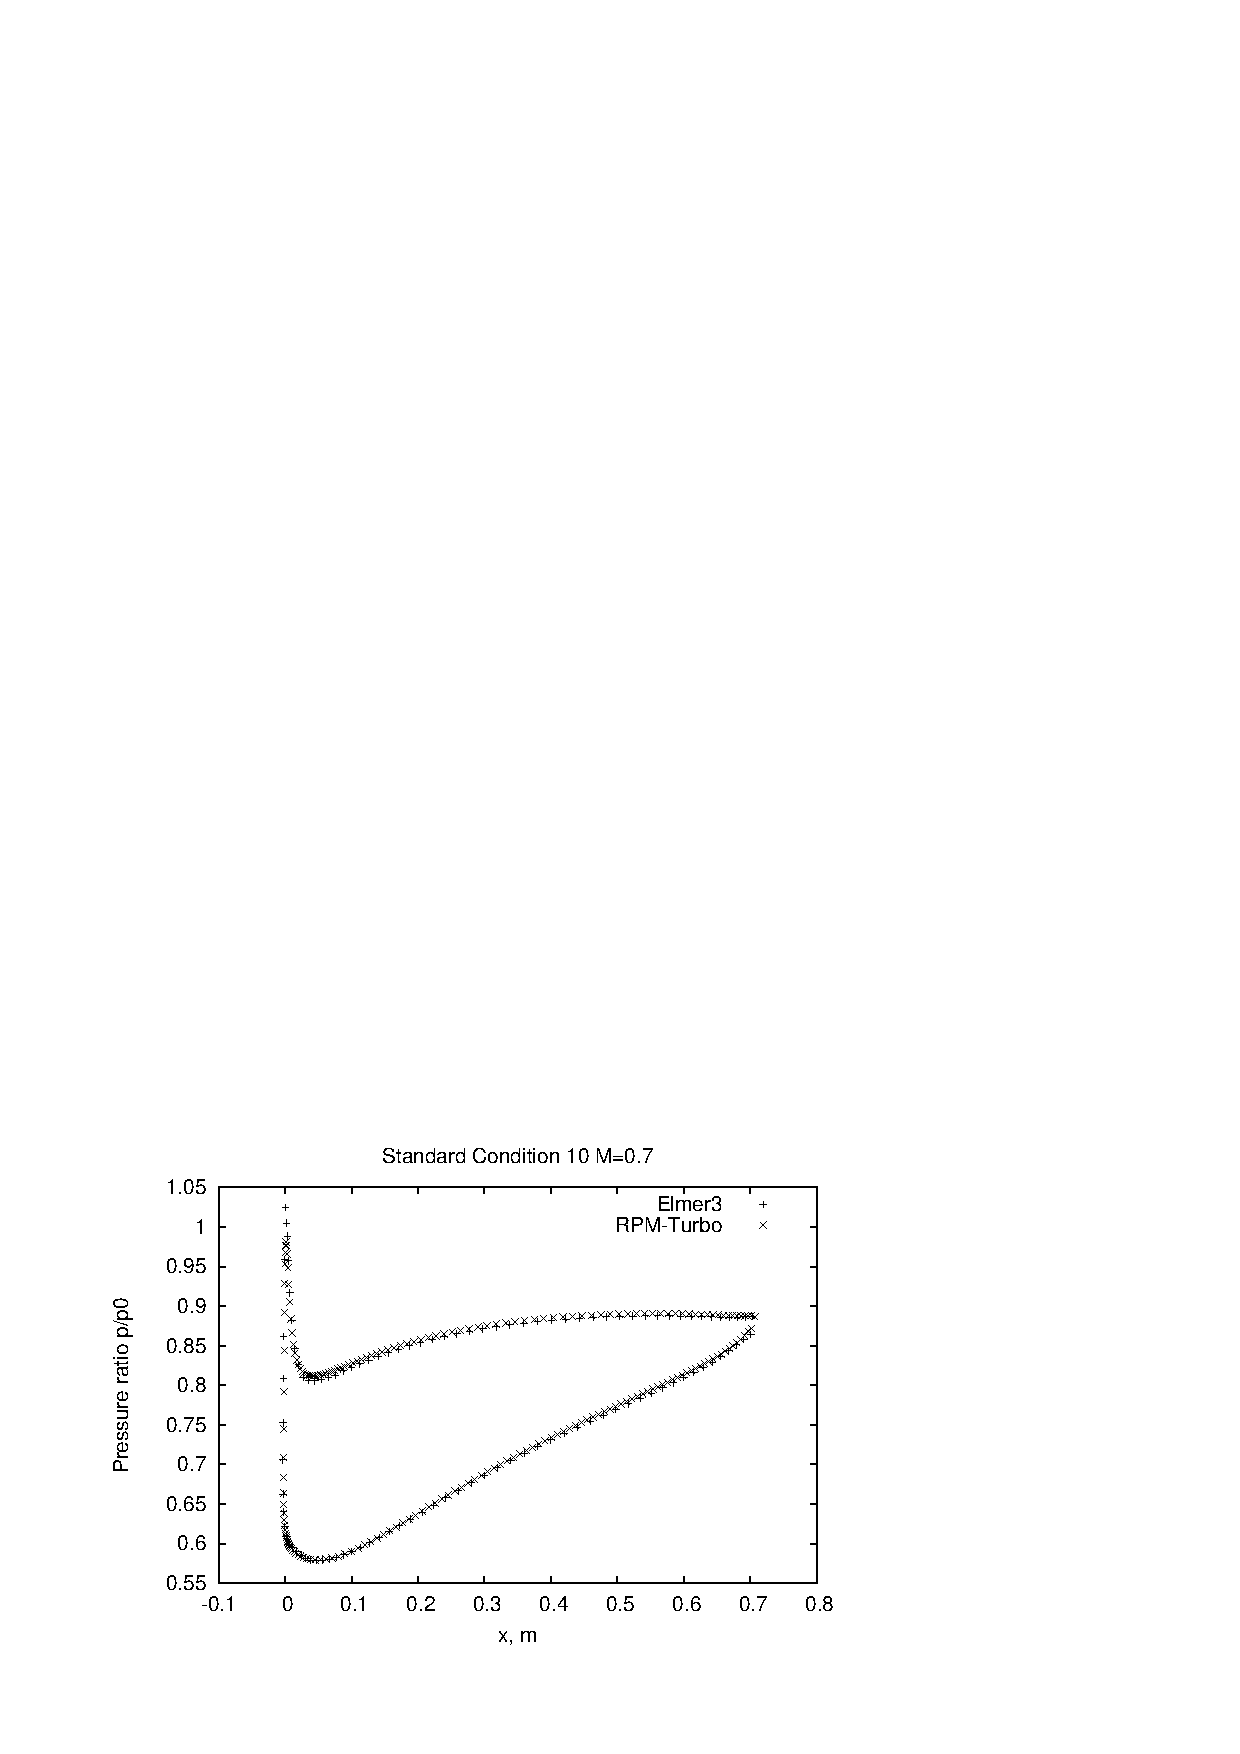
\includegraphics[width=10cm]{../2D/turbo_sc10_parametric/surface_p.pdf}
\end{center}
\caption{Pressure around the blade surface; comparison with RPM-Turbo reference data.}
\label{turbo-sc10-parametric-surface-p-fig}
\end{figure}

\subsection{Input scripts (.py)}
\topbar
\lstinputlisting[language={}]{../2D/turbo_sc10_parametric/sc10.py}
\bottombar\\
\topbar
\lstinputlisting[language={}]{../2D/turbo_sc10_parametric/sc10_blade_profile.py}
\bottombar

\subsection{Notes}
\begin{itemize}
\item Run time is approximately 11700 seconds for 280460 steps on a computer with 
      an AMD Phenom 9650 2.7\,GHz processor.

\end{itemize}
